\PassOptionsToPackage{unicode=true}{hyperref} % options for packages loaded elsewhere
\PassOptionsToPackage{hyphens}{url}
%
\documentclass[]{article}
\usepackage{lmodern}
\usepackage{amssymb,amsmath}
\usepackage{ifxetex,ifluatex}
\usepackage{fixltx2e} % provides \textsubscript
\ifnum 0\ifxetex 1\fi\ifluatex 1\fi=0 % if pdftex
  \usepackage[T1]{fontenc}
  \usepackage[utf8]{inputenc}
  \usepackage{textcomp} % provides euro and other symbols
\else % if luatex or xelatex
  \usepackage{unicode-math}
  \defaultfontfeatures{Ligatures=TeX,Scale=MatchLowercase}
\fi
% use upquote if available, for straight quotes in verbatim environments
\IfFileExists{upquote.sty}{\usepackage{upquote}}{}
% use microtype if available
\IfFileExists{microtype.sty}{%
\usepackage[]{microtype}
\UseMicrotypeSet[protrusion]{basicmath} % disable protrusion for tt fonts
}{}
\IfFileExists{parskip.sty}{%
\usepackage{parskip}
}{% else
\setlength{\parindent}{0pt}
\setlength{\parskip}{6pt plus 2pt minus 1pt}
}
\usepackage{hyperref}
\hypersetup{
            pdftitle={My fantastic R markdown},
            pdfauthor={Viki Mészáros},
            pdfborder={0 0 0},
            breaklinks=true}
\urlstyle{same}  % don't use monospace font for urls
\usepackage[margin=1in]{geometry}
\usepackage{color}
\usepackage{fancyvrb}
\newcommand{\VerbBar}{|}
\newcommand{\VERB}{\Verb[commandchars=\\\{\}]}
\DefineVerbatimEnvironment{Highlighting}{Verbatim}{commandchars=\\\{\}}
% Add ',fontsize=\small' for more characters per line
\usepackage{framed}
\definecolor{shadecolor}{RGB}{248,248,248}
\newenvironment{Shaded}{\begin{snugshade}}{\end{snugshade}}
\newcommand{\AlertTok}[1]{\textcolor[rgb]{0.94,0.16,0.16}{#1}}
\newcommand{\AnnotationTok}[1]{\textcolor[rgb]{0.56,0.35,0.01}{\textbf{\textit{#1}}}}
\newcommand{\AttributeTok}[1]{\textcolor[rgb]{0.77,0.63,0.00}{#1}}
\newcommand{\BaseNTok}[1]{\textcolor[rgb]{0.00,0.00,0.81}{#1}}
\newcommand{\BuiltInTok}[1]{#1}
\newcommand{\CharTok}[1]{\textcolor[rgb]{0.31,0.60,0.02}{#1}}
\newcommand{\CommentTok}[1]{\textcolor[rgb]{0.56,0.35,0.01}{\textit{#1}}}
\newcommand{\CommentVarTok}[1]{\textcolor[rgb]{0.56,0.35,0.01}{\textbf{\textit{#1}}}}
\newcommand{\ConstantTok}[1]{\textcolor[rgb]{0.00,0.00,0.00}{#1}}
\newcommand{\ControlFlowTok}[1]{\textcolor[rgb]{0.13,0.29,0.53}{\textbf{#1}}}
\newcommand{\DataTypeTok}[1]{\textcolor[rgb]{0.13,0.29,0.53}{#1}}
\newcommand{\DecValTok}[1]{\textcolor[rgb]{0.00,0.00,0.81}{#1}}
\newcommand{\DocumentationTok}[1]{\textcolor[rgb]{0.56,0.35,0.01}{\textbf{\textit{#1}}}}
\newcommand{\ErrorTok}[1]{\textcolor[rgb]{0.64,0.00,0.00}{\textbf{#1}}}
\newcommand{\ExtensionTok}[1]{#1}
\newcommand{\FloatTok}[1]{\textcolor[rgb]{0.00,0.00,0.81}{#1}}
\newcommand{\FunctionTok}[1]{\textcolor[rgb]{0.00,0.00,0.00}{#1}}
\newcommand{\ImportTok}[1]{#1}
\newcommand{\InformationTok}[1]{\textcolor[rgb]{0.56,0.35,0.01}{\textbf{\textit{#1}}}}
\newcommand{\KeywordTok}[1]{\textcolor[rgb]{0.13,0.29,0.53}{\textbf{#1}}}
\newcommand{\NormalTok}[1]{#1}
\newcommand{\OperatorTok}[1]{\textcolor[rgb]{0.81,0.36,0.00}{\textbf{#1}}}
\newcommand{\OtherTok}[1]{\textcolor[rgb]{0.56,0.35,0.01}{#1}}
\newcommand{\PreprocessorTok}[1]{\textcolor[rgb]{0.56,0.35,0.01}{\textit{#1}}}
\newcommand{\RegionMarkerTok}[1]{#1}
\newcommand{\SpecialCharTok}[1]{\textcolor[rgb]{0.00,0.00,0.00}{#1}}
\newcommand{\SpecialStringTok}[1]{\textcolor[rgb]{0.31,0.60,0.02}{#1}}
\newcommand{\StringTok}[1]{\textcolor[rgb]{0.31,0.60,0.02}{#1}}
\newcommand{\VariableTok}[1]{\textcolor[rgb]{0.00,0.00,0.00}{#1}}
\newcommand{\VerbatimStringTok}[1]{\textcolor[rgb]{0.31,0.60,0.02}{#1}}
\newcommand{\WarningTok}[1]{\textcolor[rgb]{0.56,0.35,0.01}{\textbf{\textit{#1}}}}
\usepackage{graphicx,grffile}
\makeatletter
\def\maxwidth{\ifdim\Gin@nat@width>\linewidth\linewidth\else\Gin@nat@width\fi}
\def\maxheight{\ifdim\Gin@nat@height>\textheight\textheight\else\Gin@nat@height\fi}
\makeatother
% Scale images if necessary, so that they will not overflow the page
% margins by default, and it is still possible to overwrite the defaults
% using explicit options in \includegraphics[width, height, ...]{}
\setkeys{Gin}{width=\maxwidth,height=\maxheight,keepaspectratio}
\usepackage[normalem]{ulem}
% avoid problems with \sout in headers with hyperref:
\pdfstringdefDisableCommands{\renewcommand{\sout}{}}
\setlength{\emergencystretch}{3em}  % prevent overfull lines
\providecommand{\tightlist}{%
  \setlength{\itemsep}{0pt}\setlength{\parskip}{0pt}}
\setcounter{secnumdepth}{0}
% Redefines (sub)paragraphs to behave more like sections
\ifx\paragraph\undefined\else
\let\oldparagraph\paragraph
\renewcommand{\paragraph}[1]{\oldparagraph{#1}\mbox{}}
\fi
\ifx\subparagraph\undefined\else
\let\oldsubparagraph\subparagraph
\renewcommand{\subparagraph}[1]{\oldsubparagraph{#1}\mbox{}}
\fi

% set default figure placement to htbp
\makeatletter
\def\fps@figure{htbp}
\makeatother

\usepackage{etoolbox}
\makeatletter
\providecommand{\subtitle}[1]{% add subtitle to \maketitle
  \apptocmd{\@title}{\par {\large #1 \par}}{}{}
}
\makeatother
\usepackage{booktabs}
\usepackage{longtable}
\usepackage{array}
\usepackage{multirow}
\usepackage{wrapfig}
\usepackage{float}
\usepackage{colortbl}
\usepackage{pdflscape}
\usepackage{tabu}
\usepackage{threeparttable}
\usepackage{threeparttablex}
\usepackage[normalem]{ulem}
\usepackage{makecell}
\usepackage{xcolor}

\title{My fantastic R markdown}
\providecommand{\subtitle}[1]{}
\subtitle{This is the cool subtitle of my document}
\author{Viki Mészáros}
\date{21/09/2021}

\begin{document}
\maketitle

{
\setcounter{tocdepth}{2}
\tableofcontents
}
\hypertarget{write-with-markdown}{%
\section{Write with Markdown}\label{write-with-markdown}}

You can easily include text to a markdown file. With two spaces\\
you can start a new paragraph.

When you include a backslash\\
you will have a new line.

You can also play around with the text you include. You can create
\textbf{bold} or \emph{italic} parts or could even \sout{strikethrough}
some words. You may need to include some superscrips
x\textsuperscript{2} or subsripts x\textsubscript{1}.

\begin{center}\rule{0.5\linewidth}{0.5pt}\end{center}

\hypertarget{headers}{%
\section{Headers}\label{headers}}

When creating documents you will most probably need to use some
headings.

\hypertarget{really-big-ones}{%
\subsection{Really big ones}\label{really-big-ones}}

\hypertarget{smaller-ones}{%
\subsubsection{Smaller ones}\label{smaller-ones}}

\hypertarget{or-even-pretty-smalls}{%
\subparagraph{Or even pretty smalls}\label{or-even-pretty-smalls}}

\begin{center}\rule{0.5\linewidth}{0.5pt}\end{center}

\hypertarget{lists}{%
\section{Lists}\label{lists}}

You can include cool ordered and unordered lists as well.

\textbf{Thing I like the most}

\begin{itemize}
\tightlist
\item
  Coding
\item
  R
\item
  The R Mentoring Class

  \begin{itemize}
  \tightlist
  \item
    Misi
  \item
    Viki
  \end{itemize}
\end{itemize}

\emph{My aims for the year}

\begin{enumerate}
\def\labelenumi{\arabic{enumi}.}
\tightlist
\item
  Become a pro in coding
\item
  Attend all R Mentoring classes
\item
  Enjoy my studies
\end{enumerate}

\begin{center}\rule{0.5\linewidth}{0.5pt}\end{center}

\hypertarget{links}{%
\section{Links}\label{links}}

When you would like to put a link in your document, you can put the
whole thing in the document, or you can also link it to a word which
looks much better.

Here is a cool website to style my markdowns.
\url{https://prettydoc.statr.me/}

Here is a cool \href{https://prettydoc.statr.me/}{website} to style my
markdowns.

\begin{center}\rule{0.5\linewidth}{0.5pt}\end{center}

\hypertarget{equations}{%
\section{Equations}\label{equations}}

During your studies you will probably need to include some equations as
well.

You can do this within your text. \(e^{i \pi} + 1 = 0\) And continue
explaining.

Or you may create a separate block.

\[E = mc^{2}\]

\begin{center}\rule{0.5\linewidth}{0.5pt}\end{center}

\hypertarget{chunk-options}{%
\section{Chunk options}\label{chunk-options}}

After text elements the other most important thing you will put into
your markdown is code.

You can include this between

There are several different options you can use within the \{\}. Without
anything the code you write will be shown and the results as well.

\begin{Shaded}
\begin{Highlighting}[]
\NormalTok{df =}\StringTok{ }\NormalTok{iris}
\KeywordTok{head}\NormalTok{(df, }\DecValTok{3}\NormalTok{)}
\end{Highlighting}
\end{Shaded}

\begin{verbatim}
##   Sepal.Length Sepal.Width Petal.Length Petal.Width Species
## 1          5.1         3.5          1.4         0.2  setosa
## 2          4.9         3.0          1.4         0.2  setosa
## 3          4.7         3.2          1.3         0.2  setosa
\end{verbatim}

With \texttt{eval=FALSE} (or \texttt{eval=F}) the code won't be
evaluated, but it will be printed out.

\begin{Shaded}
\begin{Highlighting}[]
\NormalTok{df =}\StringTok{ }\NormalTok{iris}
\KeywordTok{head}\NormalTok{(df, }\DecValTok{3}\NormalTok{)}
\end{Highlighting}
\end{Shaded}

With \texttt{echo=F} you can only show the output of the chunk but hide
the code you used to get it. This is mostly used for figures.

\begin{verbatim}
##   Sepal.Length Sepal.Width Petal.Length Petal.Width Species
## 1          5.1         3.5          1.4         0.2  setosa
## 2          4.9         3.0          1.4         0.2  setosa
## 3          4.7         3.2          1.3         0.2  setosa
\end{verbatim}

With \texttt{include=F} you can exclude the chunk. It will run in the
background. This is useful for data import or package loadings.

\begin{center}\rule{0.5\linewidth}{0.5pt}\end{center}

\hypertarget{figures}{%
\section{Figures}\label{figures}}

For example here I am only showing the fig without the codes.

\begin{verbatim}
## `geom_smooth()` using formula 'y ~ x'
\end{verbatim}

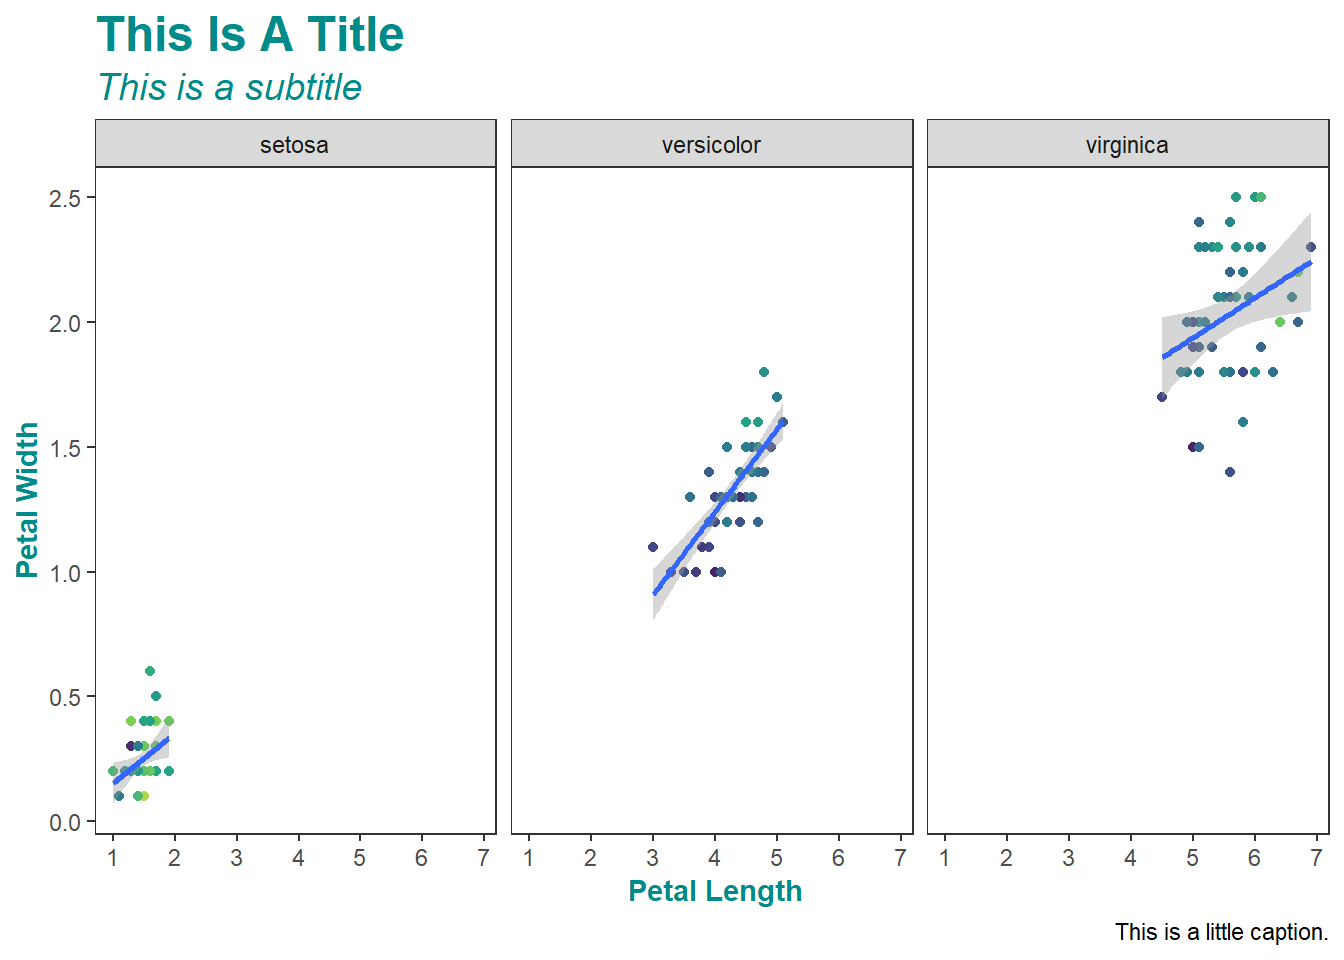
\includegraphics{Sample_markdown_files/figure-latex/iris fig-1.pdf}

Here is the code for generate the plot

\begin{Shaded}
\begin{Highlighting}[]
\KeywordTok{library}\NormalTok{(ggplot2)}

\NormalTok{p <-}\StringTok{ }\KeywordTok{ggplot}\NormalTok{(}\DataTypeTok{data=}\NormalTok{iris,}\DataTypeTok{mapping=}\KeywordTok{aes}\NormalTok{(}\DataTypeTok{x=}\NormalTok{Petal.Length,}\DataTypeTok{y=}\NormalTok{Petal.Width))}\OperatorTok{+}
\StringTok{  }\KeywordTok{geom_point}\NormalTok{(}\KeywordTok{aes}\NormalTok{(}\DataTypeTok{color=}\NormalTok{Sepal.Width))}\OperatorTok{+}
\StringTok{  }\KeywordTok{geom_smooth}\NormalTok{(}\DataTypeTok{method=}\StringTok{"lm"}\NormalTok{)}\OperatorTok{+}
\StringTok{  }\KeywordTok{scale_color_viridis_c}\NormalTok{()}\OperatorTok{+}
\StringTok{  }\KeywordTok{scale_x_continuous}\NormalTok{(}\DataTypeTok{breaks=}\DecValTok{1}\OperatorTok{:}\DecValTok{8}\NormalTok{)}\OperatorTok{+}
\StringTok{  }\KeywordTok{labs}\NormalTok{(}\DataTypeTok{title=}\StringTok{"This Is A Title"}\NormalTok{,}\DataTypeTok{subtitle=}\StringTok{"This is a subtitle"}\NormalTok{,}\DataTypeTok{x=}\StringTok{" Petal Length"}\NormalTok{, }
       \DataTypeTok{y=}\StringTok{"Petal Width"}\NormalTok{, }\DataTypeTok{caption=}\StringTok{"This is a little caption."}\NormalTok{)}\OperatorTok{+}
\StringTok{  }\KeywordTok{facet_wrap}\NormalTok{(}\OperatorTok{~}\NormalTok{Species)}\OperatorTok{+}
\StringTok{  }\KeywordTok{theme_bw}\NormalTok{()}\OperatorTok{+}
\StringTok{  }\KeywordTok{theme}\NormalTok{(}
    \DataTypeTok{axis.title=}\KeywordTok{element_text}\NormalTok{(}\DataTypeTok{color=}\StringTok{"cyan4"}\NormalTok{,}\DataTypeTok{face=}\StringTok{"bold"}\NormalTok{, }\DataTypeTok{size =} \DecValTok{11}\NormalTok{),}
    \DataTypeTok{plot.title=}\KeywordTok{element_text}\NormalTok{(}\DataTypeTok{color=}\StringTok{"cyan4"}\NormalTok{,}\DataTypeTok{face=}\StringTok{"bold"}\NormalTok{, }\DataTypeTok{size =} \DecValTok{18}\NormalTok{),}
    \DataTypeTok{plot.subtitle=}\KeywordTok{element_text}\NormalTok{(}\DataTypeTok{color=}\StringTok{"cyan4"}\NormalTok{, }\DataTypeTok{face =} \StringTok{"italic"}\NormalTok{, }\DataTypeTok{size =} \DecValTok{14}\NormalTok{),}
    \DataTypeTok{panel.grid=}\KeywordTok{element_blank}\NormalTok{(),}
    \DataTypeTok{legend.position =} \StringTok{"none"}
\NormalTok{  )}

\KeywordTok{show}\NormalTok{(p)}
\end{Highlighting}
\end{Shaded}

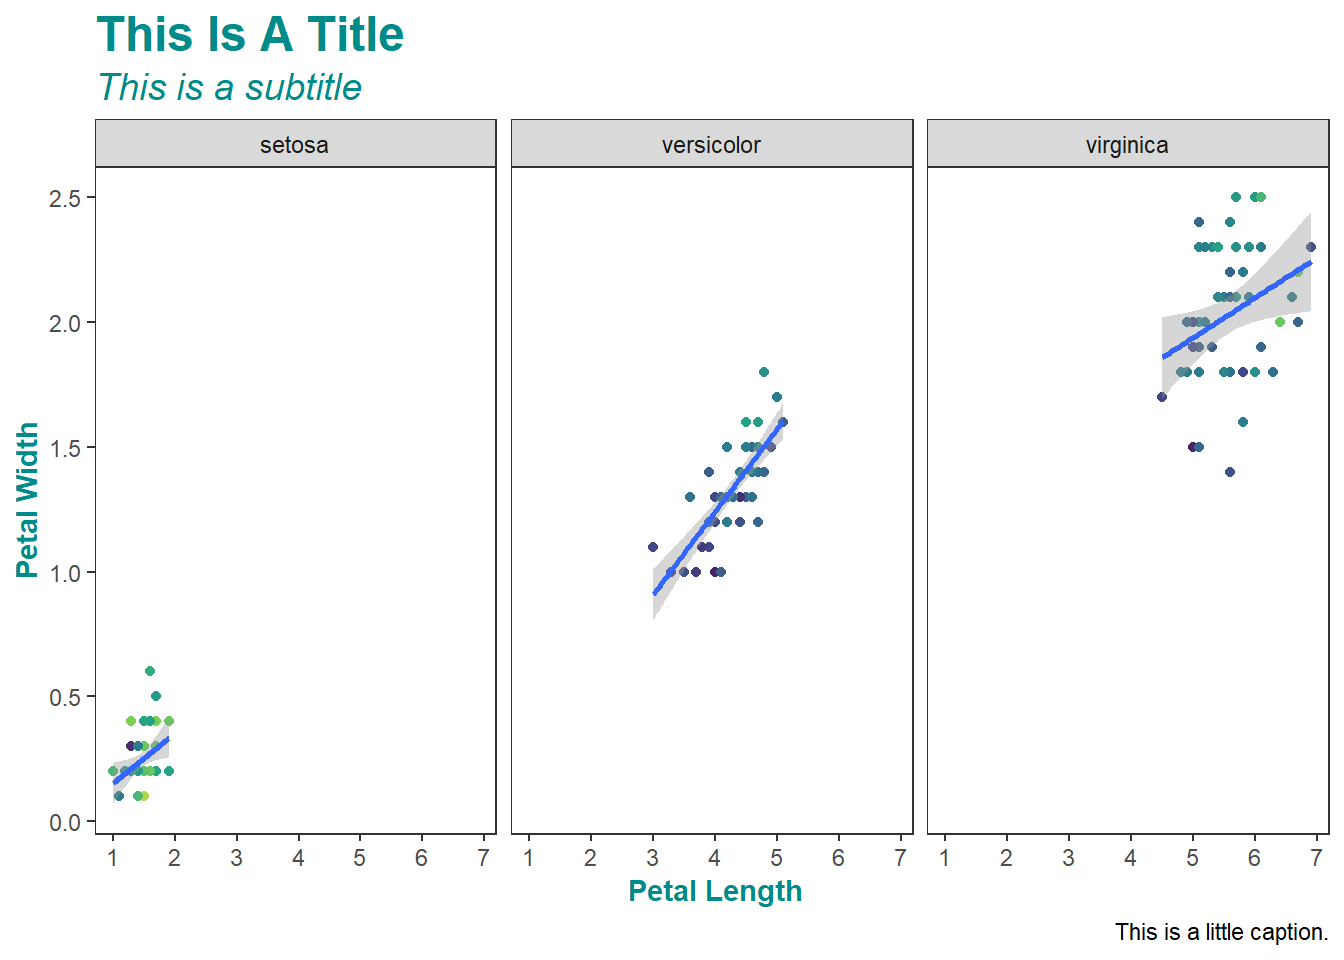
\includegraphics{Sample_markdown_files/figure-latex/unnamed-chunk-1-1.pdf}

There are two extra lines before the graph. It is also possible to hide
them. For this you can use \texttt{warning=F} to hide warning messages
(\emph{for example}: Warning: package `ggplot2' was built under R
version 4.0.5)

\begin{verbatim}
## `geom_smooth()` using formula 'y ~ x'
\end{verbatim}

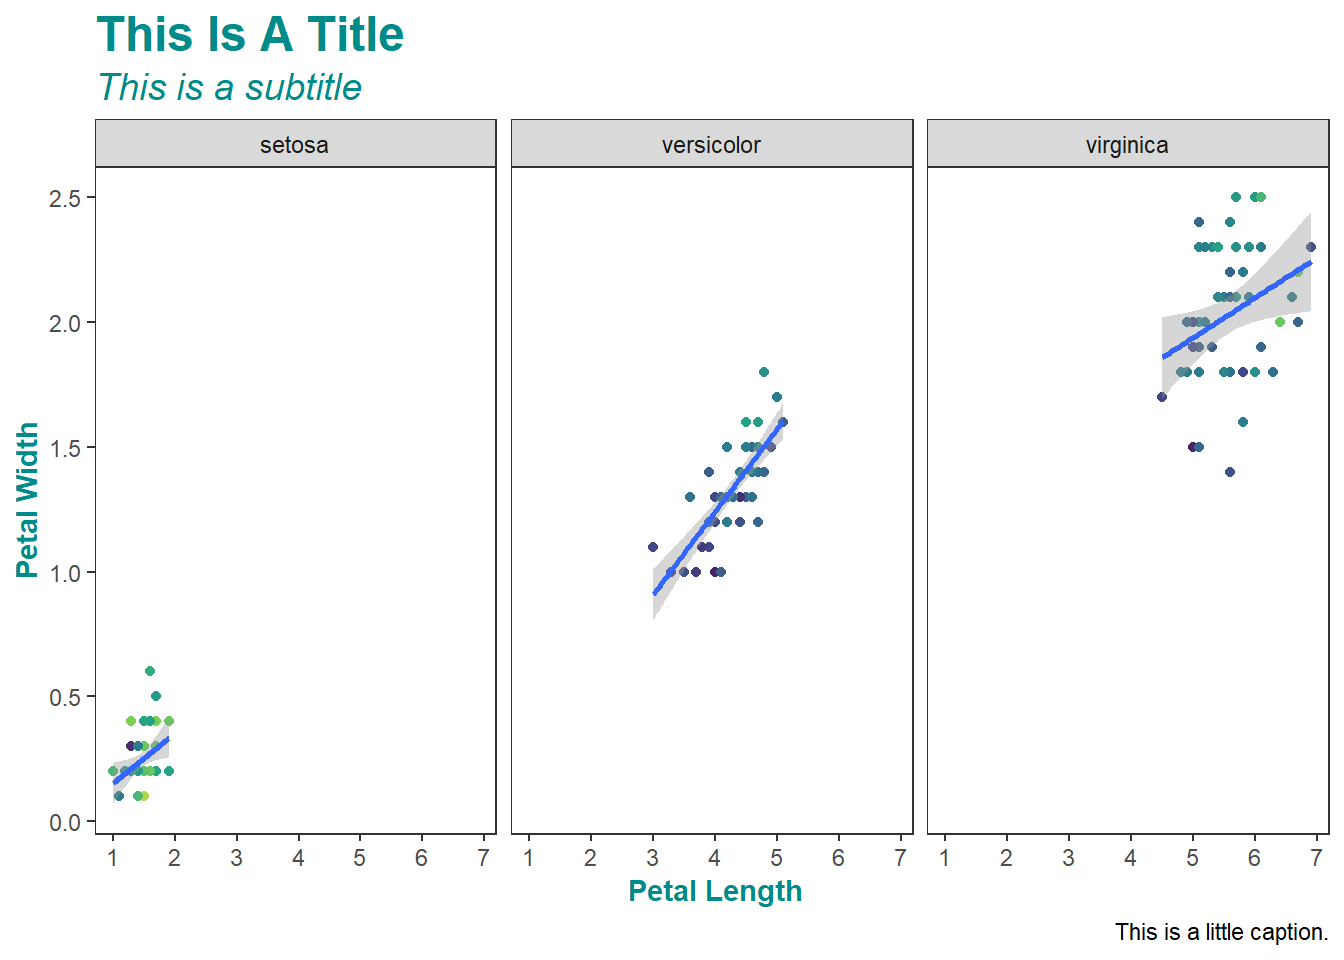
\includegraphics{Sample_markdown_files/figure-latex/unnamed-chunk-2-1.pdf}

With \texttt{message=F} you can also hide any additional messages.
(\emph{for example}: `geom\_smooth()' using formula `y \textasciitilde{}
x')

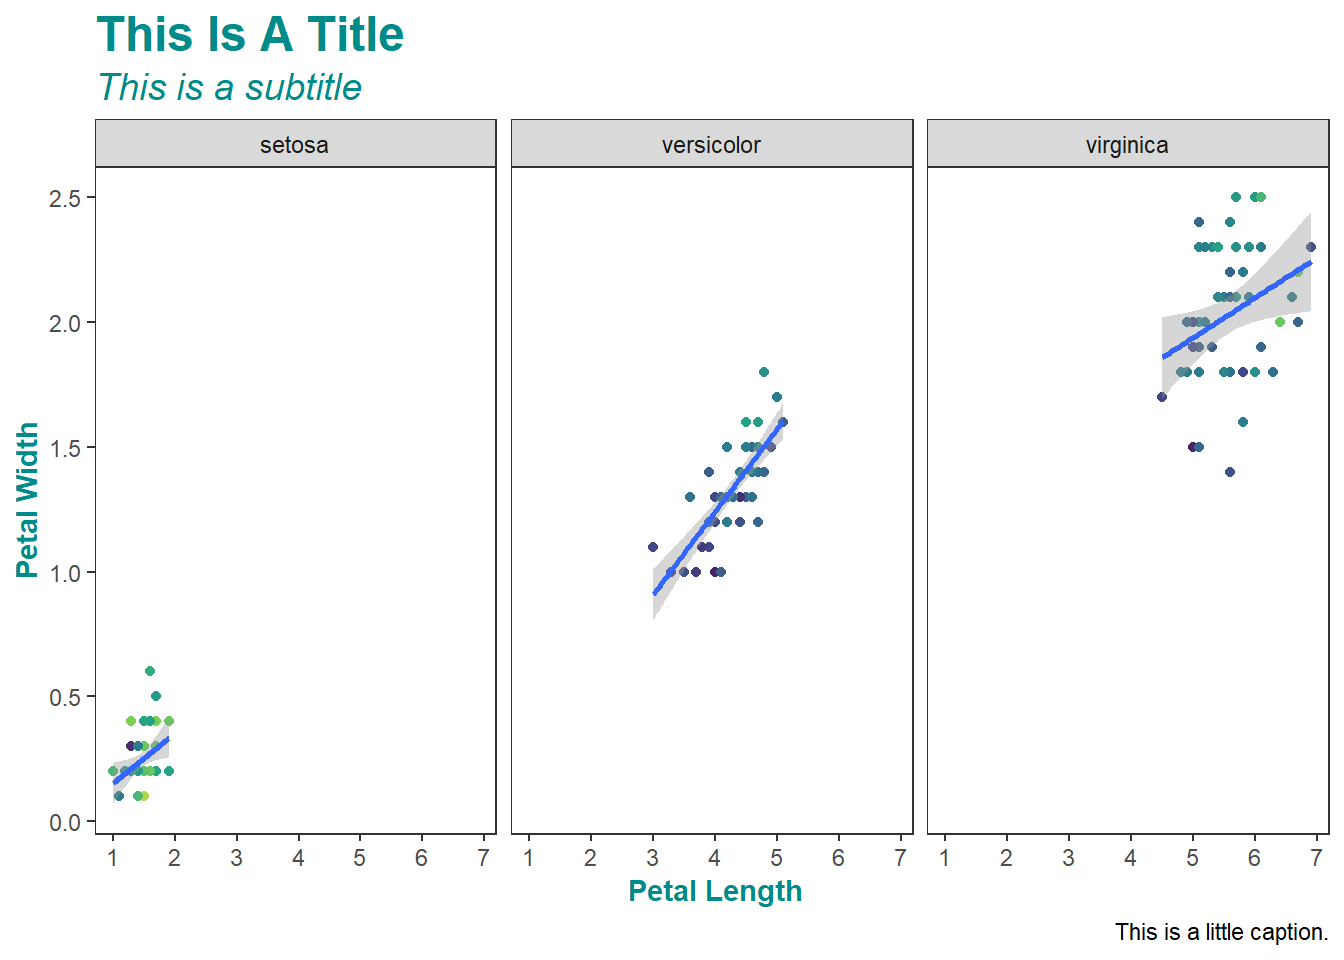
\includegraphics{Sample_markdown_files/figure-latex/unnamed-chunk-3-1.pdf}

\begin{center}\rule{0.5\linewidth}{0.5pt}\end{center}

You can also play around with the alignment of the figure.

\begin{center}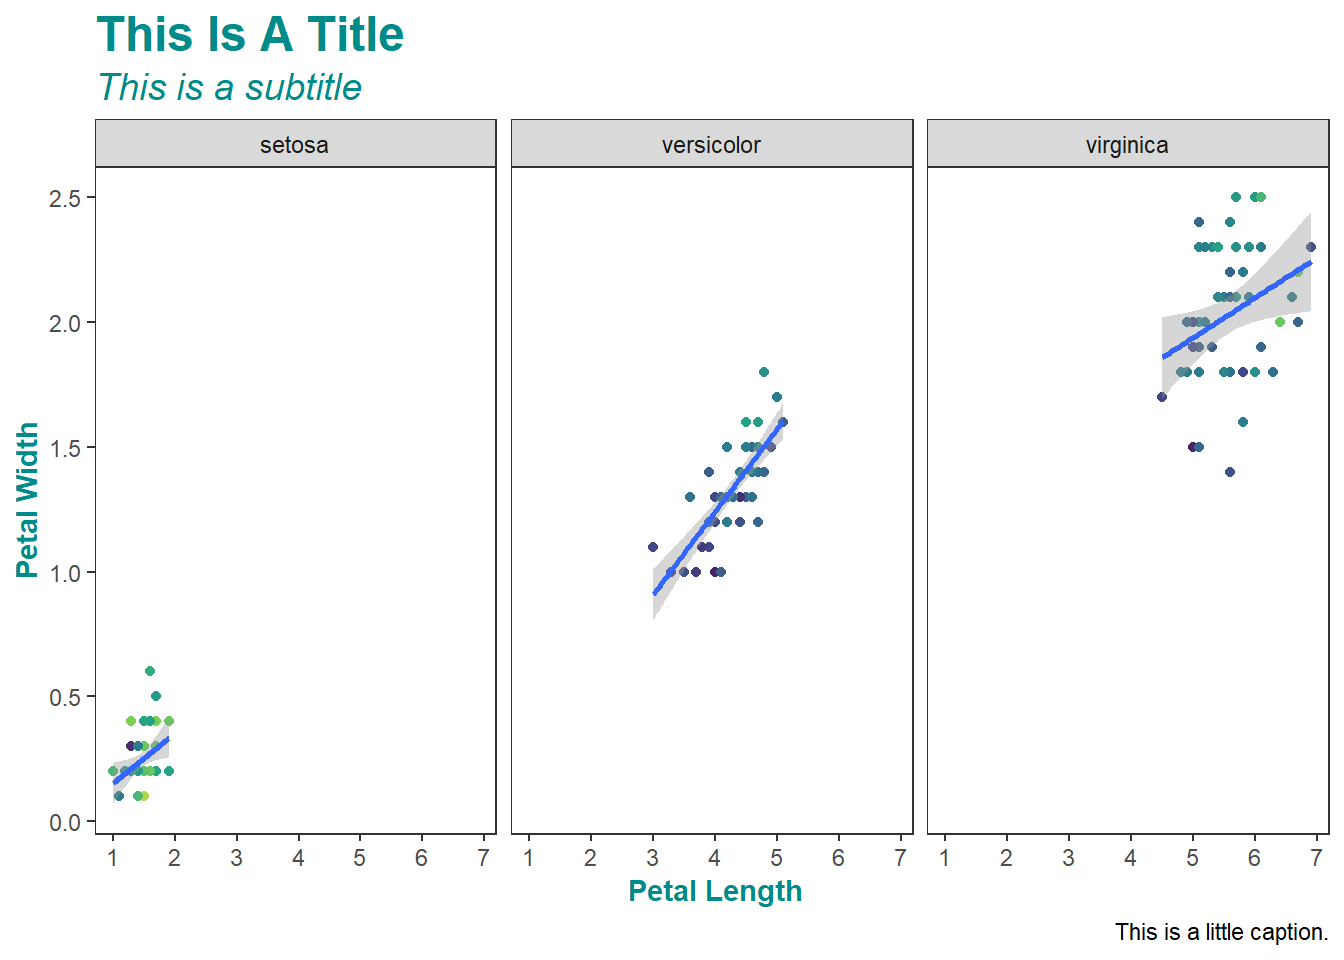
\includegraphics{Sample_markdown_files/figure-latex/unnamed-chunk-4-1} \end{center}

Or can change the size by the lines \texttt{out.width=} command. After
the equal sign you can use percentages like \emph{``50\%''} or pixel
sizes like \emph{``300px''}

\textbf{Using the measure ``50\%''}

\begin{flushright}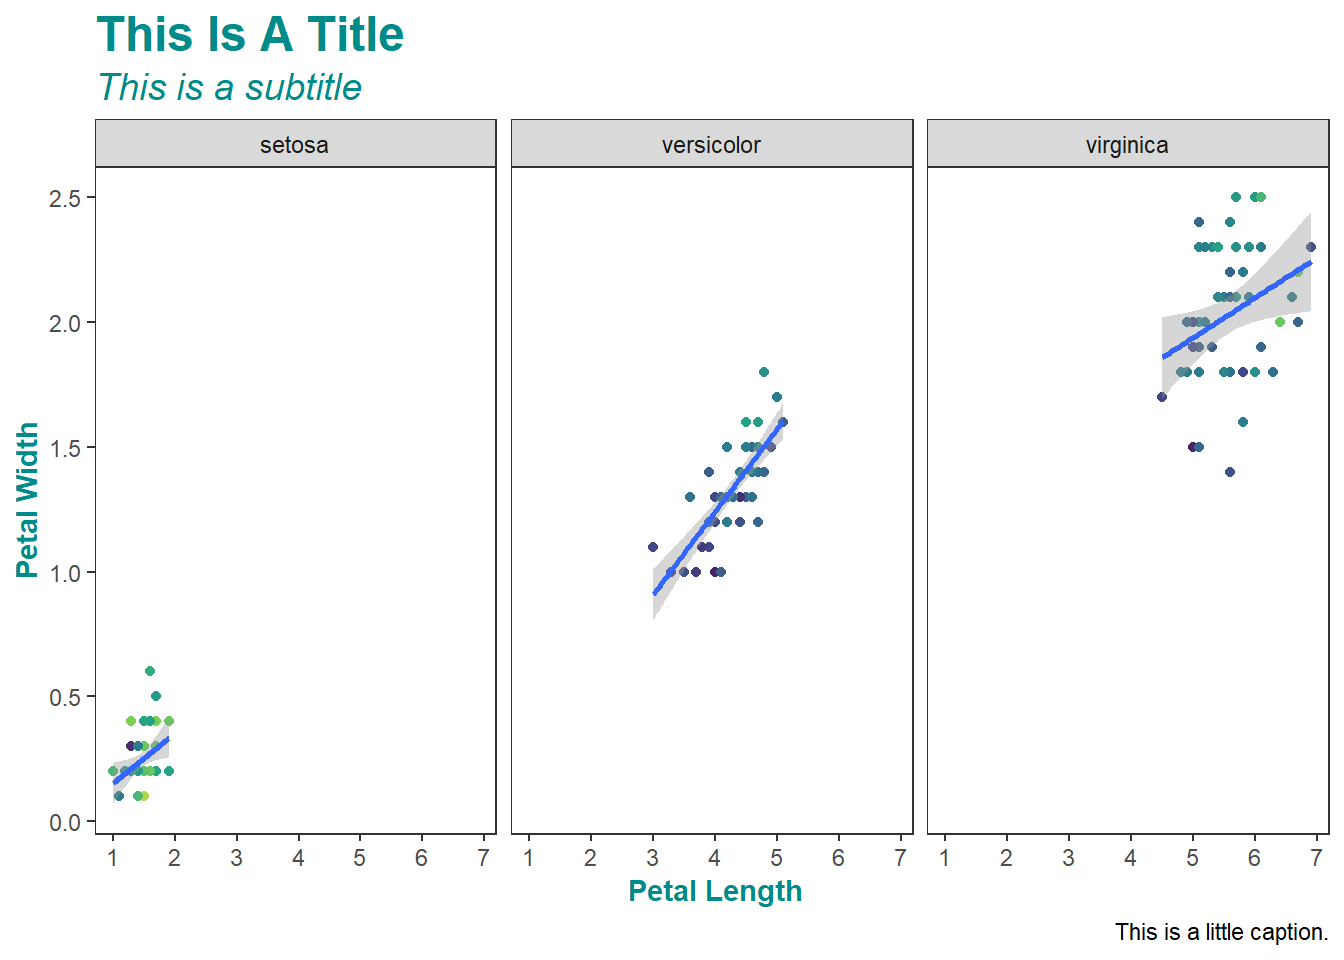
\includegraphics[width=0.5\linewidth]{Sample_markdown_files/figure-latex/unnamed-chunk-5-1} \end{flushright}

\textbf{Using the measure ``500px''}

\begin{center}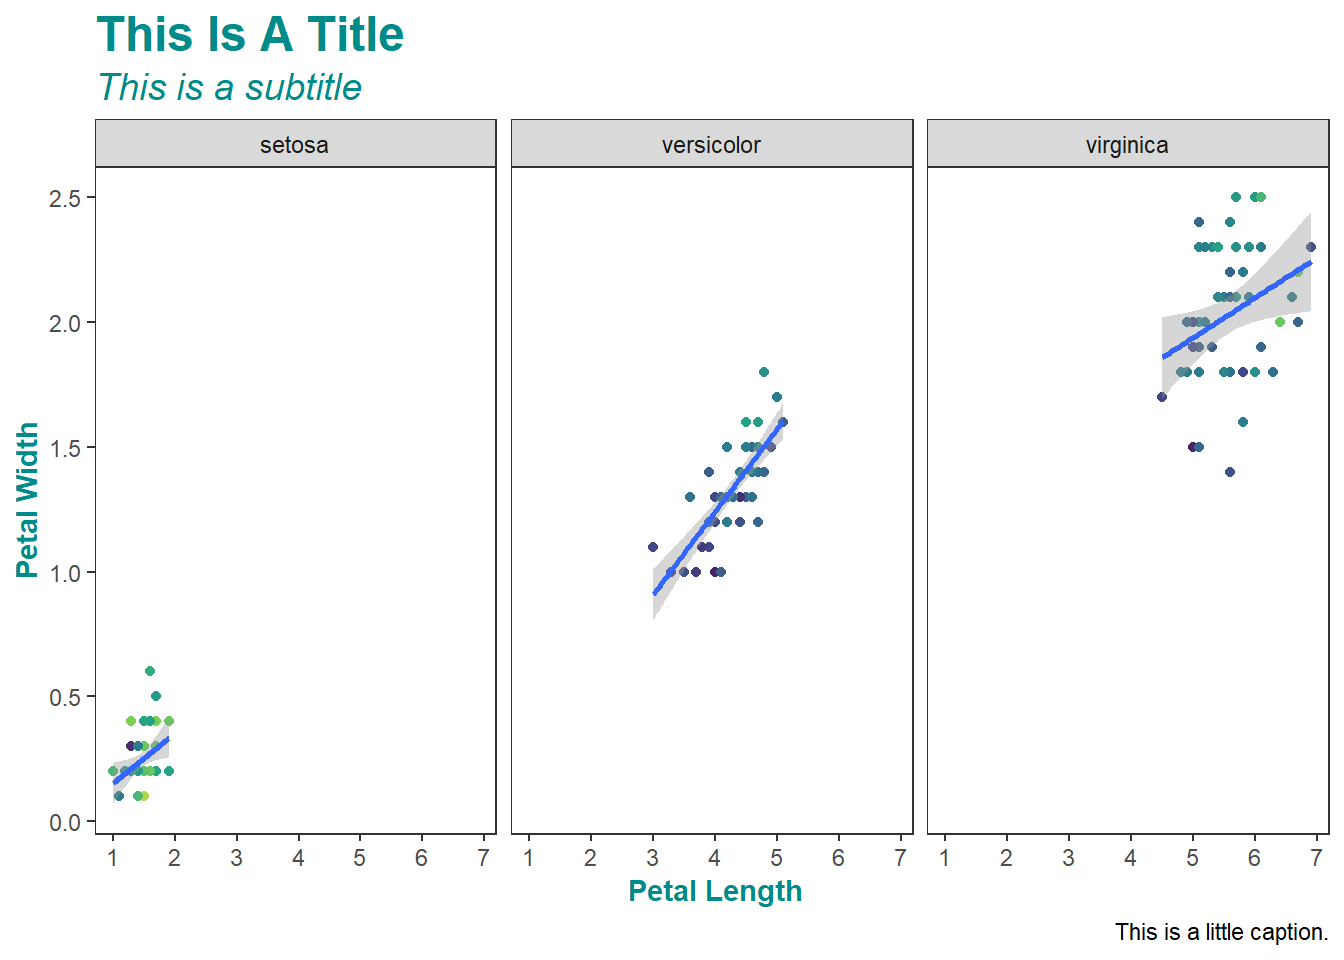
\includegraphics[width=500px]{Sample_markdown_files/figure-latex/unnamed-chunk-6-1} \end{center}

\hypertarget{tables}{%
\section{Tables}\label{tables}}

There are some extra option to show your data in a markdown. The package
I used the most was
\href{https://cran.r-project.org/web/packages/kableExtra/vignettes/awesome_table_in_html.html}{KableExtra}.

This is what the basic table would look like.

\begin{Shaded}
\begin{Highlighting}[]
\KeywordTok{head}\NormalTok{(df, }\DecValTok{3}\NormalTok{)}
\end{Highlighting}
\end{Shaded}

\begin{verbatim}
##   Sepal.Length Sepal.Width Petal.Length Petal.Width Species
## 1          5.1         3.5          1.4         0.2  setosa
## 2          4.9         3.0          1.4         0.2  setosa
## 3          4.7         3.2          1.3         0.2  setosa
\end{verbatim}

This is how it looks with kableExtra.

\begin{Shaded}
\begin{Highlighting}[]
\KeywordTok{library}\NormalTok{(kableExtra)}
\end{Highlighting}
\end{Shaded}

\begin{verbatim}
## Warning: package 'kableExtra' was built under R version 3.6.3
\end{verbatim}

\begin{Shaded}
\begin{Highlighting}[]
\KeywordTok{head}\NormalTok{(df, }\DecValTok{3}\NormalTok{) }\OperatorTok\StringTok{ }
\StringTok{  }\KeywordTok{kbl}\NormalTok{() }
\end{Highlighting}
\end{Shaded}

\begin{tabular}[t]{r|r|r|r|l}
\hline
Sepal.Length & Sepal.Width & Petal.Length & Petal.Width & Species\\
\hline
5.1 & 3.5 & 1.4 & 0.2 & setosa\\
\hline
4.9 & 3.0 & 1.4 & 0.2 & setosa\\
\hline
4.7 & 3.2 & 1.3 & 0.2 & setosa\\
\hline
\end{tabular}

You can add different styles.

\begin{Shaded}
\begin{Highlighting}[]
\KeywordTok{head}\NormalTok{(df, }\DecValTok{3}\NormalTok{) }\OperatorTok\StringTok{ }
\StringTok{  }\KeywordTok{kbl}\NormalTok{() }\OperatorTok\StringTok{ }
\StringTok{  }\KeywordTok{kable_classic}\NormalTok{(}\DataTypeTok{full_width =}\NormalTok{ F)}
\end{Highlighting}
\end{Shaded}

\begin{table}
\centering
\begin{tabular}[t]{r|r|r|r|l}
\hline
Sepal.Length & Sepal.Width & Petal.Length & Petal.Width & Species\\
\hline
5.1 & 3.5 & 1.4 & 0.2 & setosa\\
\hline
4.9 & 3.0 & 1.4 & 0.2 & setosa\\
\hline
4.7 & 3.2 & 1.3 & 0.2 & setosa\\
\hline
\end{tabular}
\end{table}

Or even some interactive features like hovering.

\begin{Shaded}
\begin{Highlighting}[]
\KeywordTok{head}\NormalTok{(df, }\DecValTok{3}\NormalTok{) }\OperatorTok\StringTok{ }
\StringTok{  }\KeywordTok{kbl}\NormalTok{() }\OperatorTok\StringTok{ }
\StringTok{  }\KeywordTok{kable_paper}\NormalTok{(}\KeywordTok{c}\NormalTok{(}\StringTok{"striped"}\NormalTok{, }\StringTok{"hover"}\NormalTok{), }\DataTypeTok{full_width =}\NormalTok{ F)}
\end{Highlighting}
\end{Shaded}

\begin{table}
\centering
\begin{tabular}[t]{r|r|r|r|l}
\hline
Sepal.Length & Sepal.Width & Petal.Length & Petal.Width & Species\\
\hline
5.1 & 3.5 & 1.4 & 0.2 & setosa\\
\hline
4.9 & 3.0 & 1.4 & 0.2 & setosa\\
\hline
4.7 & 3.2 & 1.3 & 0.2 & setosa\\
\hline
\end{tabular}
\end{table}

There are some additional packages you can use to format your tables
nicely.

\begin{itemize}
\tightlist
\item
  \textbf{flextable}
\item
  \textbf{gt}
\item
  \textbf{kable}
\end{itemize}

\hypertarget{styles}{%
\section{Styles}\label{styles}}

To add some extra flavor to your docs you can use different themes. For
this the easiest is to use \href{https://bootswatch.com/}{Bootswatch}.
To change the styles you just need to replace \emph{``flatly''} in the
header to one of the names you can see on the website.

Another way is to use \href{https://prettydoc.statr.me/}{Prettydoc}. For
this you can check their website and see how this works.

\end{document}
